% -*- latex -*-
% FILE: "/home/evmik/jobs/wm/2012_spring_Analog_Electronics_252/final_exam/questions/bjt_amplifier.tex"
% LAST MODIFICATION: "Tue, 01 May 2012 01:18:46 -0400 (evmik)"
% (C) 2011 by Eugeniy Mikhailov, <evgmik@gmail.com>
% $Id:$

\question{}
	Consider the circuit shown below \\
	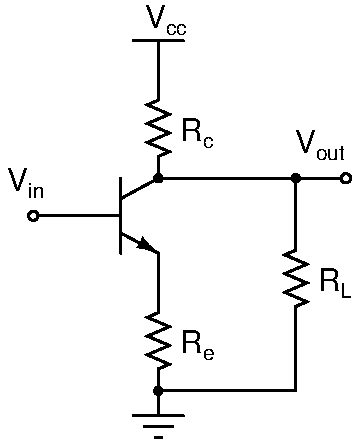
\includegraphics[height=2in]{./schematics/npn_common_emitter_amplifier}\\
	\begin{parts}
		\part[10]
		Derive the expression for the output voltage $V_{out}$, in terms of
		$V_{in}, V_{cc}, R_c, R_e,$ and  the base to emitter voltage drop $V_{be}$.
		Assume that $\beta=200$. Also assume that   the load resistor ($R_L$) is large enough and does not affect the circuit. 

		\vskip 1.5in
		$V_{out}=$
		\part[5]
		What is the small signal gain of this circuit?

		\vskip 0.5in
		$G=$
		\part[5]
		Assume that   the load resistor ($R_L$) is large enough and does not affect the circuit. 
		If $R_c/R_e=10$, $V_{be}=.6$~V and $V_{cc}=15$~V, what is
		the maximum and minimum DC
		input voltage $V_{in}$ at which this circuit  is still not saturated or railing?

		\vskip 1.0in
		$V_{{in}_{min}}=$ \hspace{2in} 
		$V_{{in}_{max}}=$
		\bonuspart[5]
		What is the output impedance of this circuit? {\bf Stating it is not
		enough, show the derivation!}

		\vskip 1.0in
		$Z_{out}=$
	\end{parts}
	\pagebreak
